\subsection{Life Cycle Smart Contract}
\label{subsec:lifecycle}

\begin{figure}[ht]
	\centering
	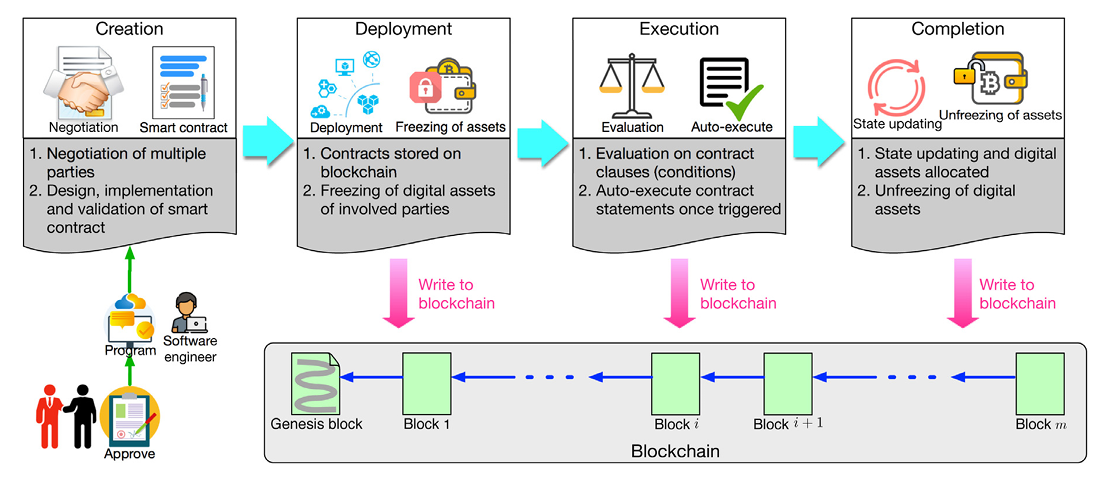
\includegraphics[width=0.7\textwidth]{resources/chapter-2/sc-lifecycle.png}
	\caption{\textit{Life cycle} dari Smart Contract \parencite{zheng2020overview}}
	\label{image:sc-lifecycle}
\end{figure}

\textit{Life cycle} dari sebuah Smart Contract terdiri dari empat fase seperti pada ilustrasi di Gambar \ref{image:sc-lifecycle}:

\begin{enumerate}
	\item \textit{Creation}: negosiasi antar pihak untuk menyepakati ketentuan dari kontrak dalam \textit{natural language}, dan translasi menjadi Smart Contracts.
	\item \textit{Deployment}: kontrak yang sudah divalidasi dapat disimpan ke dalam blockchain, menjadikannya tidak bisa dimodifikasi.
	\item \textit{Execution}: Setelah \textit{deployment}, klausa kontraktual akan dimonitor, dan saat kondisi yang sesuai dengan yang terdefinisi dalam Smart Contract, maka prosedur kontrak akan dieksekusi secara otomatis.
	\item \textit{Completion}: Setelah eksekusi, \textit{state} baru dari semua pihak akan diperbarui sesuai dengan hasil dari transaksi yang terjadi dan disimpan ke dalam blockchain.
\end{enumerate}